\subsection{RQ4: What semantic and implementation evidence does the trace expose?}

\begin{figure}[t]
\centering
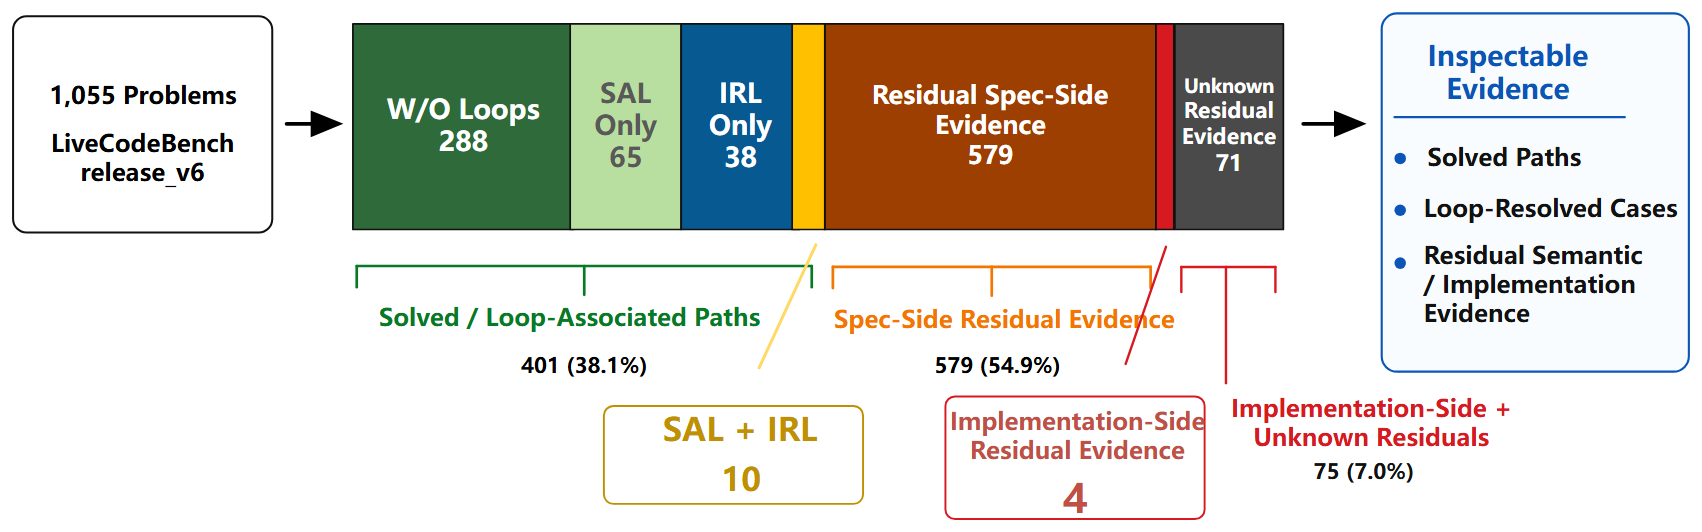
\includegraphics[width=\linewidth]{pics/trace_evidence_cn.png}
\caption{Final-aligned trace evidence.}
\label{fig:trace}
\end{figure}

Figure~\ref{fig:trace} aligns traces with final outcomes. The 401 solved programs comprise 288 paths without loop-associated change, 65 with SAL-associated change, 38 with IRL-associated change, and 10 with both. The remaining traces contain 579 specification-side labels, 4 implementation-side labels, and 71 unknowns. A balanced 36-sample audit obtains 58.3\% strict and 61.1\% relaxed agreement; Appendix~\ref{app:trace-audit} gives the detailed calibration.

\noindent\textit{Answer to RQ4.}
The trace exposes semantic and implementation evidence absent from direct generation, but it supports rather than replaces human analysis.

Together, the results support observable, reusable semantic contracts: SAL exposes semantic-state movement and IRL records verifier-level progress.
